\subsection{Sharp feature detection}

We further demonstrate the effectiveness of our neighborhood segmentation algorithm on sharp feature detection, which is a fundamental problem in geometry analysis.
%
The sharp features are usually detected as the intersection of multiple piecewise smooth surfaces.
%%
%Therefor the intersection of smooth patches produced by can be used to sharp feature detection.
%
Rejecting the pseudo features from real features challenges existing feature extraction methods, since they both are close to the intersection with similar local information, and the difference between the closeness is hard to distinguish.
%
Previous algorithms usually use multi-scale scheme or anisotropic neighborhood selection to extract feature points \cite{PaulyKG03, DanielsHOS07, WeberHH10, ParkLL12}.
%
However, these methods still could not effectively distinguish them by only using distance information.
%
Taking use of the neighborhood segmentation based on subspace structure, we design the following feature extraction method.

%%%%%%%%%%%%%%%%%%%%%%%%%%%%%%%%%%%%%%%%%%%%%%%%%%%%%%
%%%%%%%%%%%%%%%%%%%%%%%%%%%%%%%%%%%%%%%%%%%%%%%%%%%%%%%
%We believe that the true feature points are among the candidate feature points.
%
For each candidate feature point $p_{i}$, we  segment its neighborhood into some subneighborhoods and fit a plane for each.
%
Then we compute the residuals between these fitting planes and $p_{i}$.
%
If there is more than one residual which is less than the threshold $\tau_{feature}$, we consider $p_{i}$ as a feature point.
%
It is worth noting that because we use average residual to define the $\tau_{f}$, we set $\tau_{feature} = 2 \times \tau_{f}$.


%%%%%%%%%%%%%%%%%%%%%%%%%%%%%%%%%%%%%%%%%%%%%%%%%%%%%%
%%%%%%%%%%%%%%%%%%%%%%%%%%%%%%%%%%%%%%%%%%%%%%%%%%%%%%%
To assess the quality of sharp features detected by the method, we test it on synthetic models with random noise and compare it with the recent work~\cite{ParkLL12} (MSTV).
%
%Since the noise of feature detection is usually smaller than normal estimation,
The parameters $S$, $S^{*}$, $K$ and $r$ of our algorithm are choose as $S=20$, $S^{*}=60$, $K=10$ and $r=4$ for all tests in this section.

%\begin{figure}[htbp]
%\begin{center}
%    \begin{tabular}{c c c}
%        \includegraphics[width=0.3\linewidth]{fandisk_00} &
%        \includegraphics[width=0.3\linewidth]{ploy_original_343_409} &
%        \includegraphics[width=0.33\linewidth]{flower_original_343_409}\\
%        \includegraphics[width=0.3\linewidth]{fandisk_00_f} &
%        \includegraphics[width=0.3\linewidth]{ploy_feature_343_409} &
%        \includegraphics[width=0.33\linewidth]{flower_feature_343_409}
%    \end{tabular}
%    \caption{Sharp feature detection results.\label{fig:noise_free_feature}}
%\end{center}
%\end{figure}
\begin{figure}[htbp]
\begin{center}
    \begin{tabular}{c c c}
        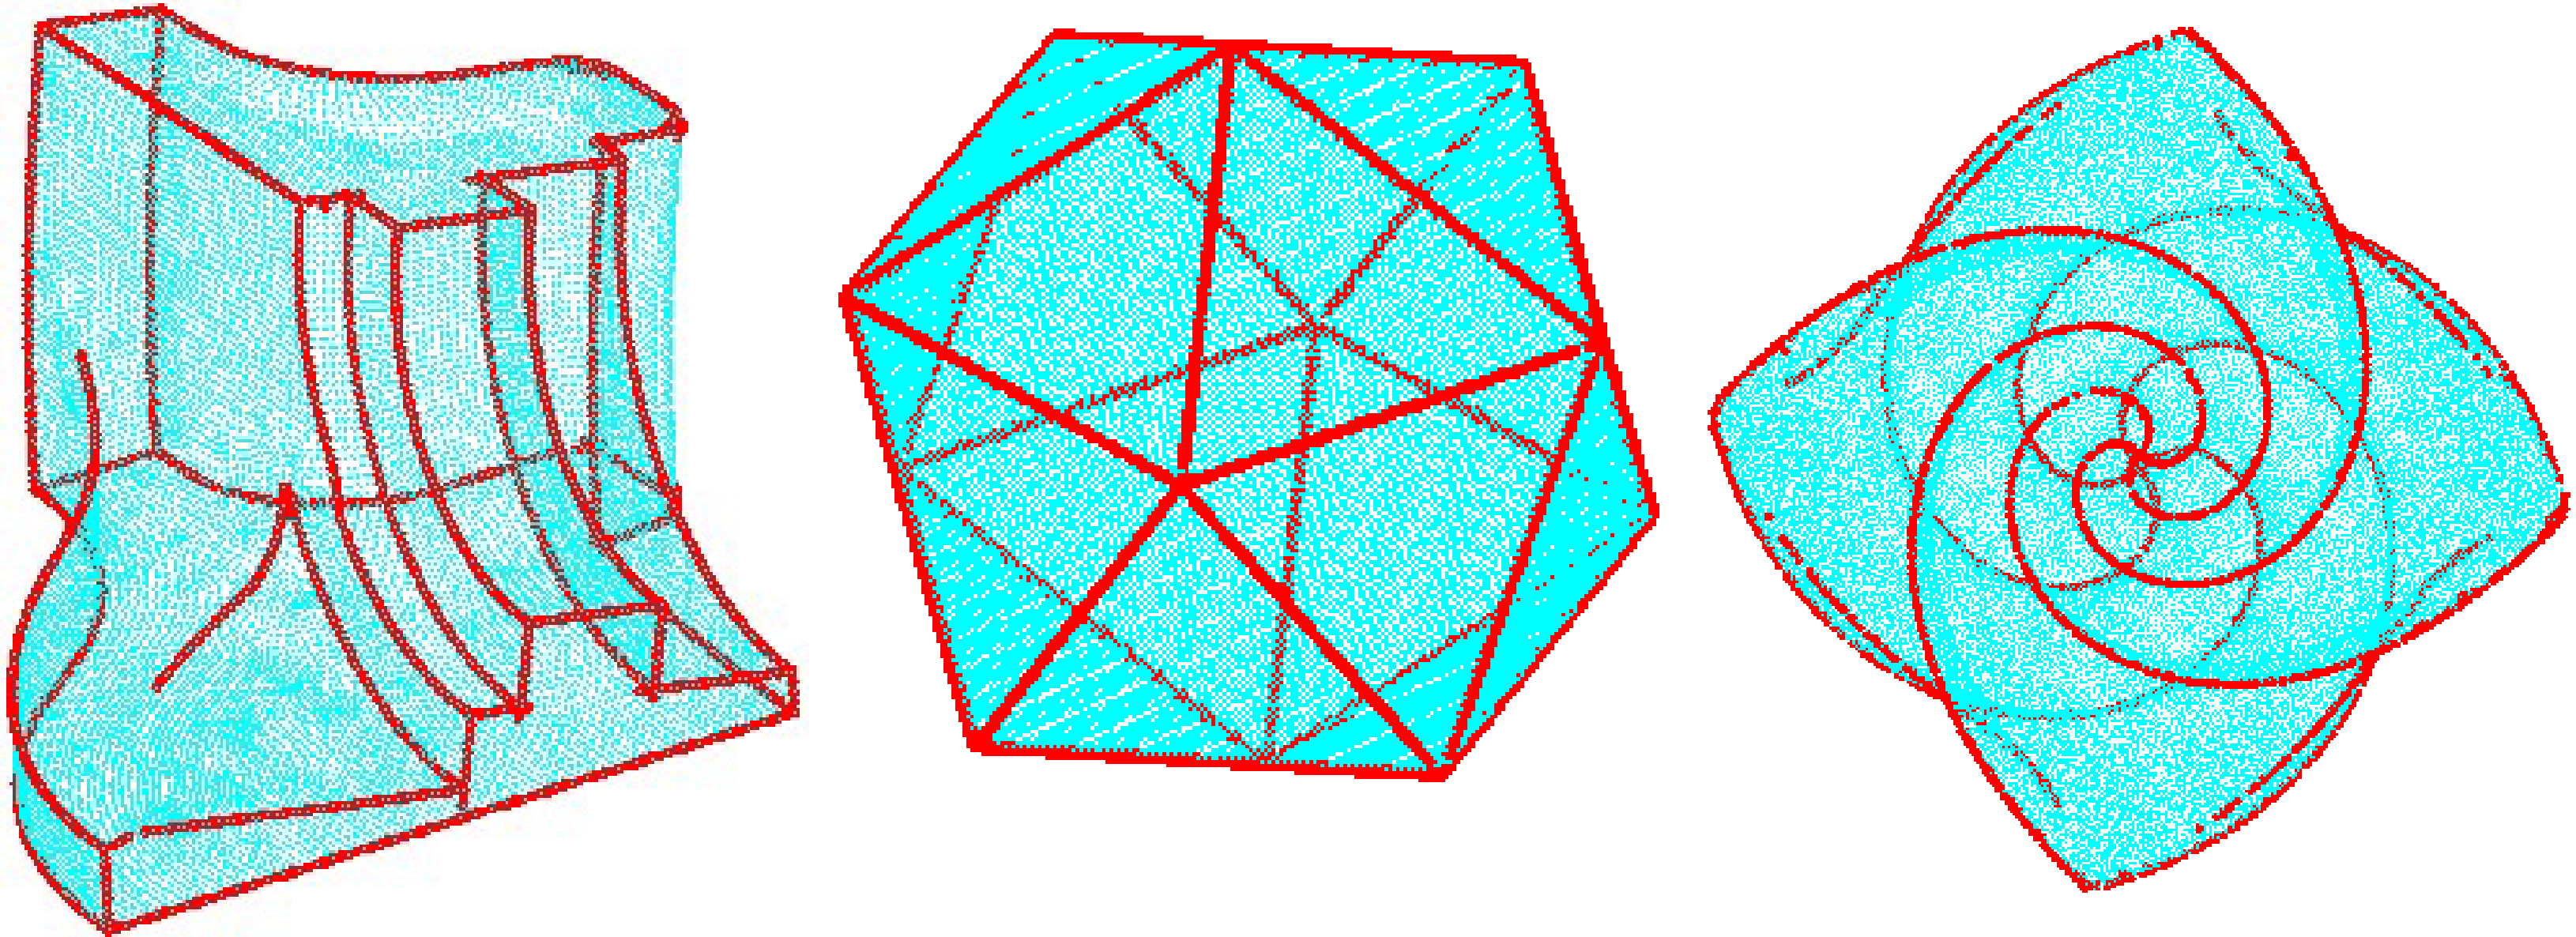
\includegraphics[width=1\linewidth]{noise_clear_feature}
    \end{tabular}
    \caption{Sharp feature detection results.\label{fig:noise_free_feature}}
\end{center}
\end{figure}
Detection results of three different models are show in Fig. \ref{fig:noise_free_feature}.
%
For these noise-free models, our method achieves almost perfect detection results, although the shapes are complex. There are Fandisk model, Icosahedron model which has corners with five adjoining planes, and Flower model where sharp features are jaggy.
%although the shapes in Fig. \ref{fig:noise_free_feature} are complex. There are \jj{...}. \jj{remove figure for weak feature}
%
We can see that our method can detect the weak features well, especially in the Flower model.


%%%%%%%%%%%%%%%%%%%%%%%%%%%%%%%%%%%%%%%%%%%%%%%%%%%%%%
%%%%%%%%%%%%%%%%%%%%%%%%%%%%%%%%%%%%%%%%%%%%%%%%%%%%%%%
In order to demonstrate the robustness of our method to noise, the results of Fandisk and Smooth-feature models are shown in \fig \ref{fig:noise} and \fig \ref{fig:compare_feature}, which are perturbed by centered Gaussian noise with the standard deviation of $10\%$ and $20\%$ average distance between points, respectively.
%Our method is robust against noise, as shown in \fig \jj{? and ?}.
%Two scales of centered Gaussian noise with the standard deviation of $10\%$ and $20\%$ average distance between points are added to the Fandisk and ? models.
%
As illustrated in \fig \ref{fig:noise}, our method is able to detect the sharp features in different noise scale for the Fandisk model.
%
Moreover, the weak features are recovered perfectly.
%
The visual comparison between the recent method MSTV and our method is given in
\fig \ref{fig:compare_feature}.
%
MSTV can not restore weak features perfectly and some weak feature points at the top of the model are missing, as shown on the top of  \fig \ref{fig:compare_feature}.
%
%The results provided by Park et al. \jj {per} are shown in Fig. \jj {fig} and \jj {fig}.
%
%The method of \jj {fig} could not restore weak features perfectly and some weak feature vertices at the top of the model are missing.
%
While evidence from the bottom of~\fig~\ref{fig:compare_feature} demonstrates that our method is capable of recovering more weak feature points to a large extent.

\begin{figure}[htcb]
  \centering
  \begin{tabular}{c c c c}
        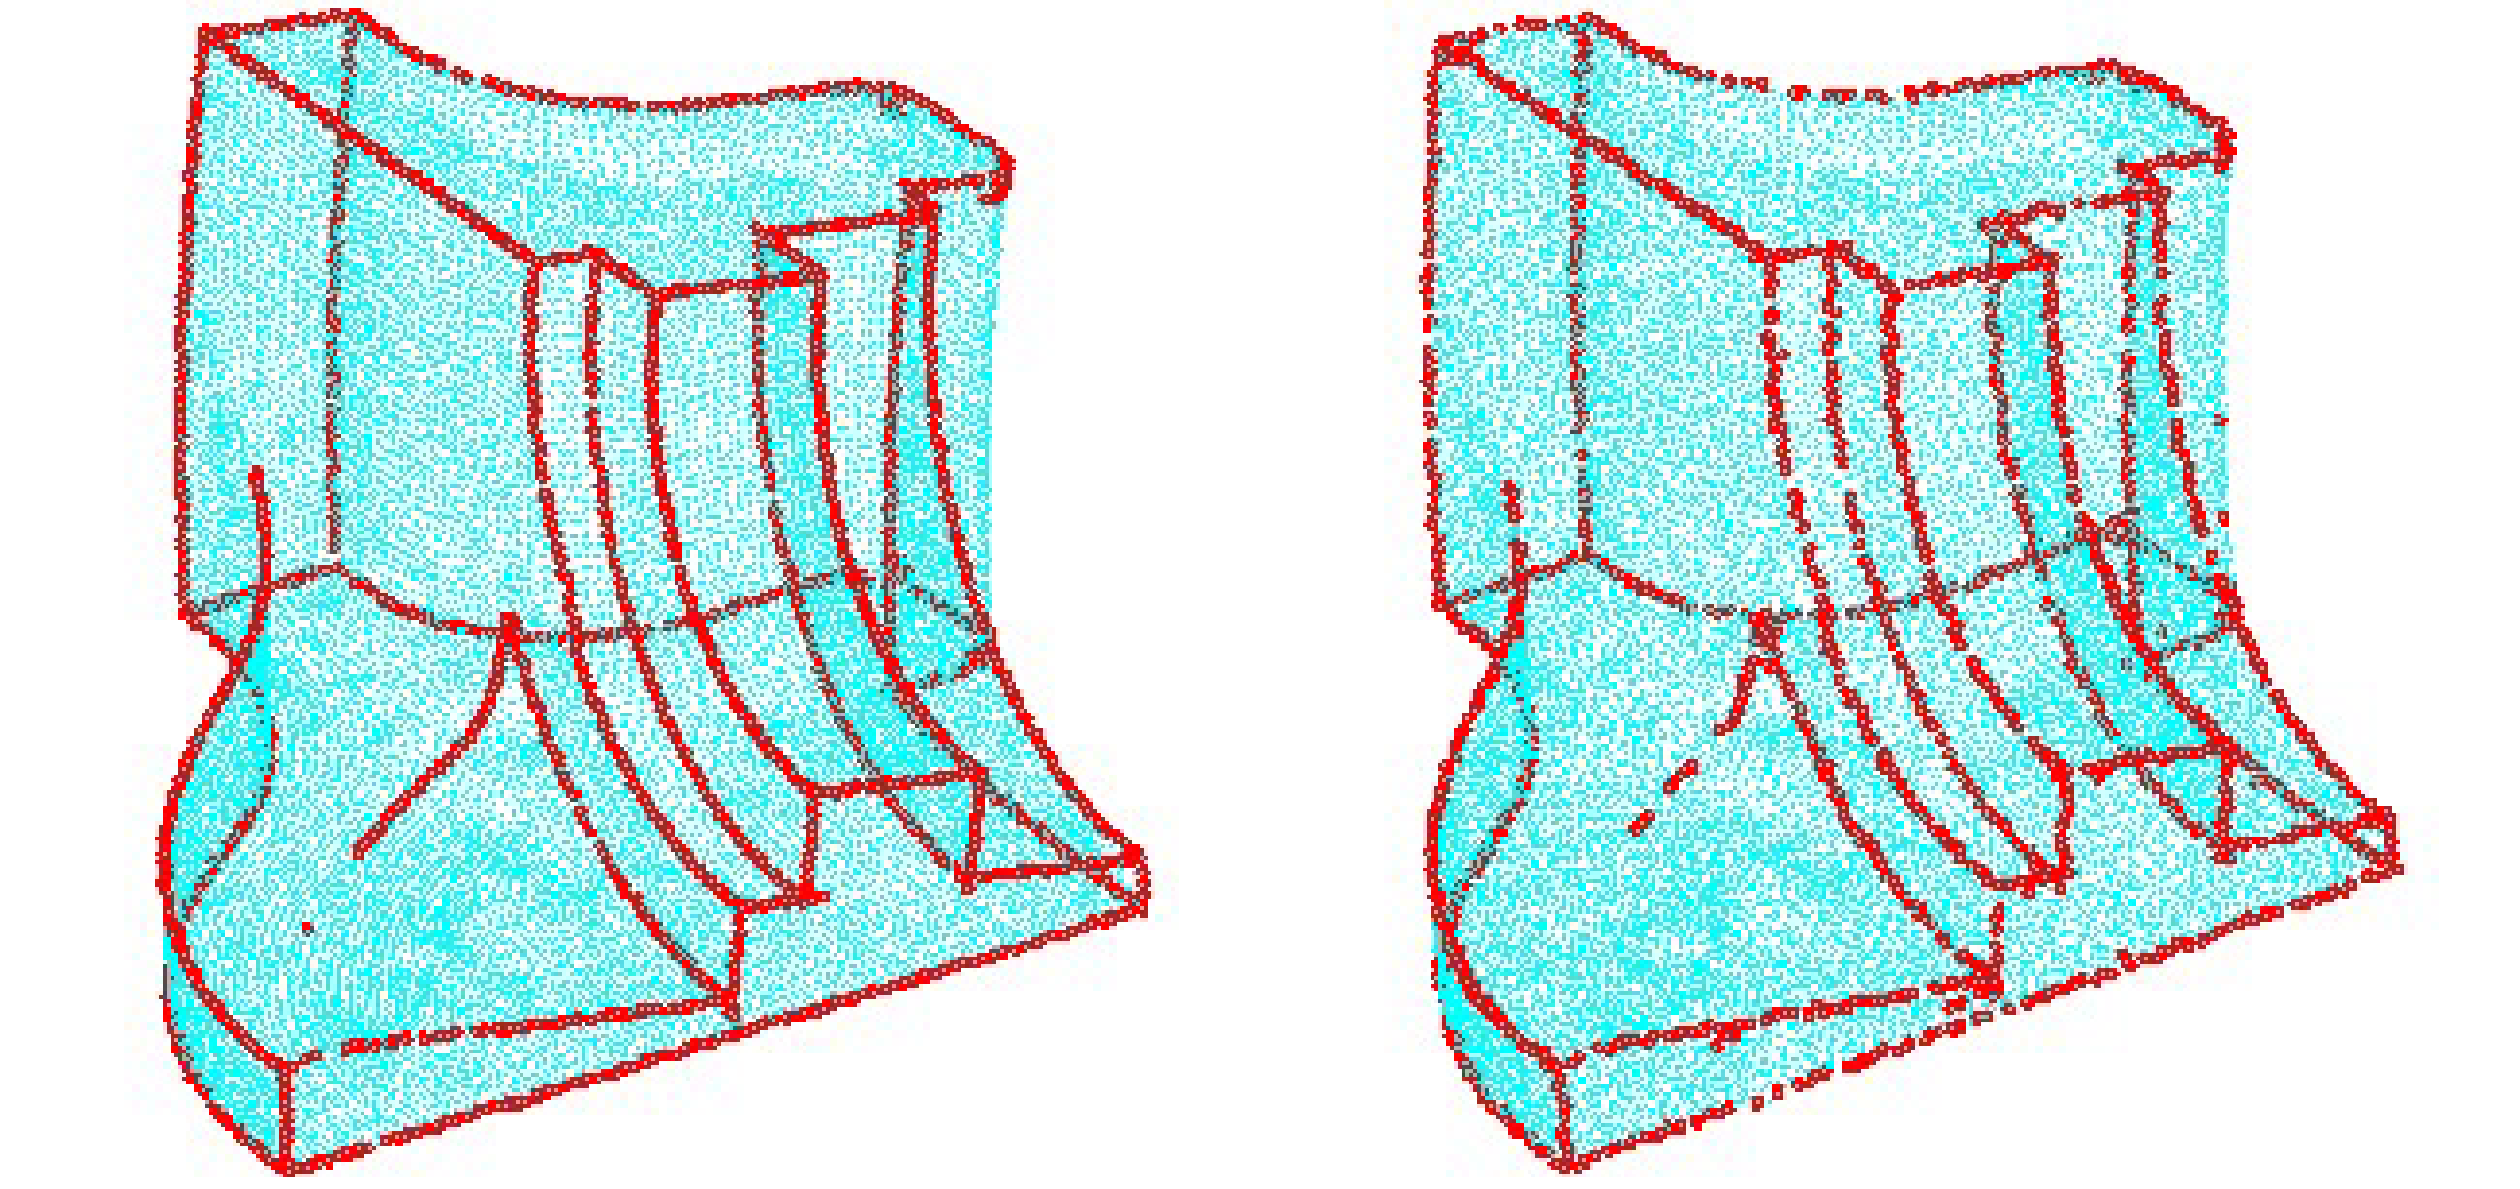
\includegraphics[width=1\linewidth]{fandisk_noise}
    \end{tabular}
  \caption{\label{fig:noise}
   Sharp feature detection results for the Fandisk model with $10\%$ (left) and $20\%$ (right) Gaussian noise.
   }
\end{figure}
\begin{figure}[htbp]
\begin{center}
    \begin{tabular}{c c }
        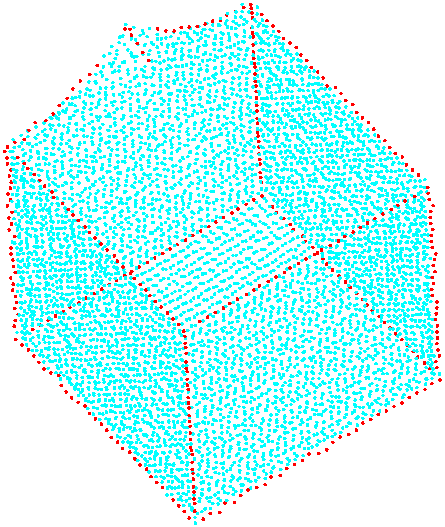
\includegraphics[width=0.4\linewidth]{smooth_10_mv} &
        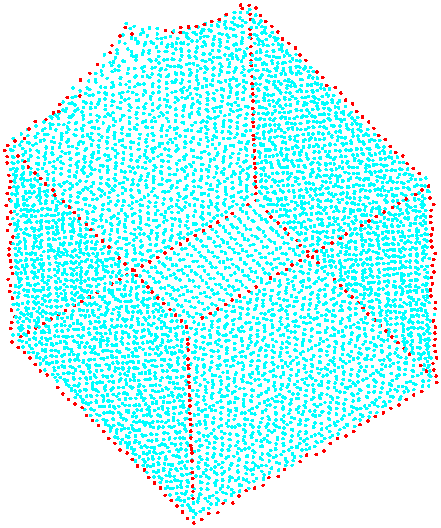
\includegraphics[width=0.4\linewidth]{smooth_20_mv} \\
        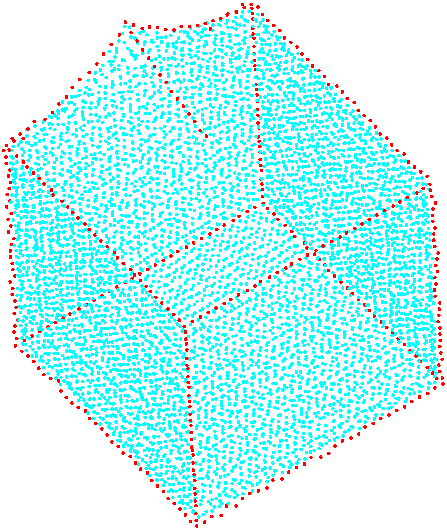
\includegraphics[width=0.4\linewidth]{smooth_10_our} &
        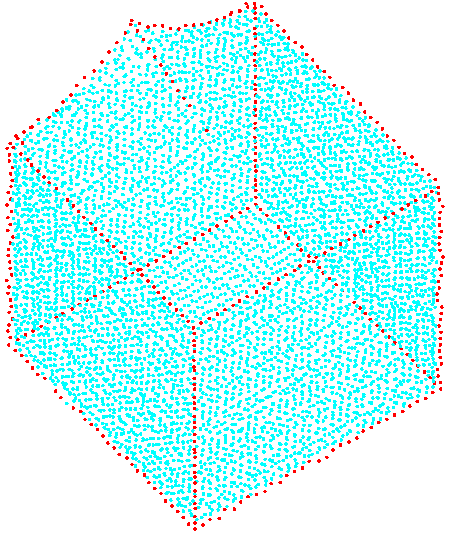
\includegraphics[width=0.4\linewidth]{smooth_20_our}
    \end{tabular}
    \caption{The sharp feature detect results by MSTV (top) and our method (bottom). Left: Smooth-feature model with $10\%$ Gaussian noise. Right: Smooth-feature model with $20\%$ Gaussian noise. \label{fig:compare_feature}}
\end{center}
\end{figure}
